\section{Camera Configuration and Post-Processing}\label{app:camera_configuration_and_postprocessing}

In order to improve success of sim-to-real transfer, the quality of visual observations is of great importance. However, the default configuration of the utilised D435 camera produced a very noisy depth map with many holes. Primary reason for this is the utilised workspace setup that consisted of a reflective surface inside a laboratory with large amount of ambient illumination. Not only does the polished metallic surface of the workspace result in a specular reflection of ceiling lights, the pattern projected by the laser emitter of the camera is completely reflected. Lack of such pattern results in limited material texture of the surface, which further decreases the attainable depth quality.

To improve quality of the raw depth map, few steps are taken. First, automatic expose of the camera's IR sensors is configured for a region of interest that covers only the workspace. This significantly reduces hot-spot clipping caused by the specular reflection, which in turn decreases the amount of holes. To mitigate noise, spatial and temporal filters are applied to the depth image. In order to achieve best results, these filters are applied to a corresponding disparity map with a high resolution of~1280~\(\times\)720~px at~30~FPS. Furthermore, the depth map is clipped only to depth rage of interest in order to reduce computational load. Once filtered, the image is decimated to a more manageable resolution of~320~\(\times\)180~px and converted to a point cloud, which can then be converted to an octree. Post-processed point cloud can be seen in \autoref{app_fig:camera_config_and_post_processing}.

\setcounter{figure}{0}
\begin{figure}[ht]
    \centering
    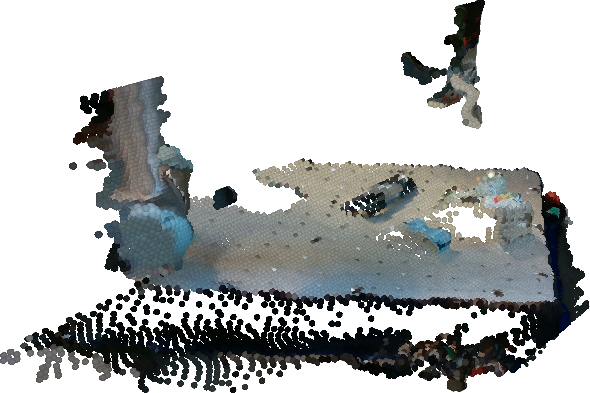
\includegraphics[width=1.0\textwidth]{experimental_evaluation/real_processed_point_cloud.png}
    \caption{Point cloud of the workspace used in real-world to evaluate sim-to-real transfer. This point cloud is subsequently used to create octree observations.}
    \label{app_fig:camera_config_and_post_processing}
\end{figure}
